\documentclass[11pt]{article}
\usepackage[margin=1in]{geometry}
\usepackage{graphicx}
\usepackage{amsmath}
\usepackage{booktabs}

\title{A Finite Intercept Correction Calculation}
\author{Anonymous}
\date{}

\begin{document}
\maketitle

\begin{abstract}
This teaching note organizes fixed-slope intercept fitting into a checkable sequence of parameter identification, loss minimization, arithmetic verification, and evaluation tracing. Five supplied observations satisfy $y=2x+3$, with baseline predictions $2x$. Their residual mean and median equal $3$, giving exact agreement after correction. At corrections $0$, $1.5$, and $3$, mean squared errors are $9$, $2.25$, and $0$. Separate algebraic arguments identify the mean and median as squared-loss and absolute-loss minimizers. Observation rows, a table, two figures, and bundled figure sources connect the calculation to its reported artifacts.
\end{abstract}

\section{Introduction}

This worked exercise targets introductory regression readers familiar with averages, absolute values, and squared error. Its instructional design aligns four checks: identify what is fitted, derive the loss-specific correction, reconstruct the reported errors, and trace which targets enter fitting and scoring. Each check has a corresponding equation, observation row, or diagram path that readers can inspect.

The supplied inputs are $x=(-2,-1,0,1,2)$, targets $y_i=2x_i+3$, and fixed predictions $2x_i$. Their constant residuals expose the exact-agreement condition. The learning objectives distinguish this condition from loss minimization: readers derive mean and median optimality separately, then explain their coincidence in the supplied calculation. The contribution is the organization of this finite demonstration into an explicit audit sequence.

\section{Related Work}

Residual analysis examines discrepancies after fitting \cite{Anscombe1963ExaminationAnalysis}. Here, the complete residual vector makes every reported error reconstructible. The formulation is intercept-only regression of those residuals on a constant, with $2x_i$ retained as a known offset. Regression through the origin instead estimates coefficients while omitting an intercept \cite{Eisenhauer2003RegressionThrough}; identifying the fitted parameter distinguishes these settings.

Friedman's additive-fitting treatment includes least-squares and least-absolute-deviation criteria \cite{Friedman2001GreedyFunction}. Here, the additive component is a single constant, allowing direct proofs for both losses. Apparent-error analysis \cite{Efron1986HowBiased} supplies the interpretation of the diagram's observation-reuse path.

\section{Method}
\subsection{Finite Setup and Mean-Residual Correction}

Define
\[
\hat y_i^{(0)}=2x_i,\qquad
r_i=y_i-\hat y_i^{(0)},\qquad
\bar r=\frac{1}{5}\sum_{i=1}^{5}r_i,\qquad
\hat y_i(b)=2x_i+b.
\]
Only $b$ is fitted. Least squares minimizes
$\sum_i[y_i-(2x_i+b)]^2=\sum_i(r_i-b)^2$.
For any five residuals,
\begin{equation}
\frac{1}{5}\sum_{i=1}^{5}(b-r_i)^2
=
\underbrace{\frac{1}{5}\sum_{i=1}^{5}(r_i-\bar r)^2}_{\text{minimum squared error}}
+(b-\bar r)^2.
\label{eq:decomposition}
\end{equation}
Expanding $b-r_i=(b-\bar r)-(r_i-\bar r)$ eliminates the cross term because $\sum_i(r_i-\bar r)=0$.
Thus $b=\bar r$ uniquely minimizes squared error. Exact agreement additionally requires every centered residual to vanish. In the supplied calculation, $r_i=\bar r=3$, so this condition holds.

\begin{figure}[!htbp]
    \centering
    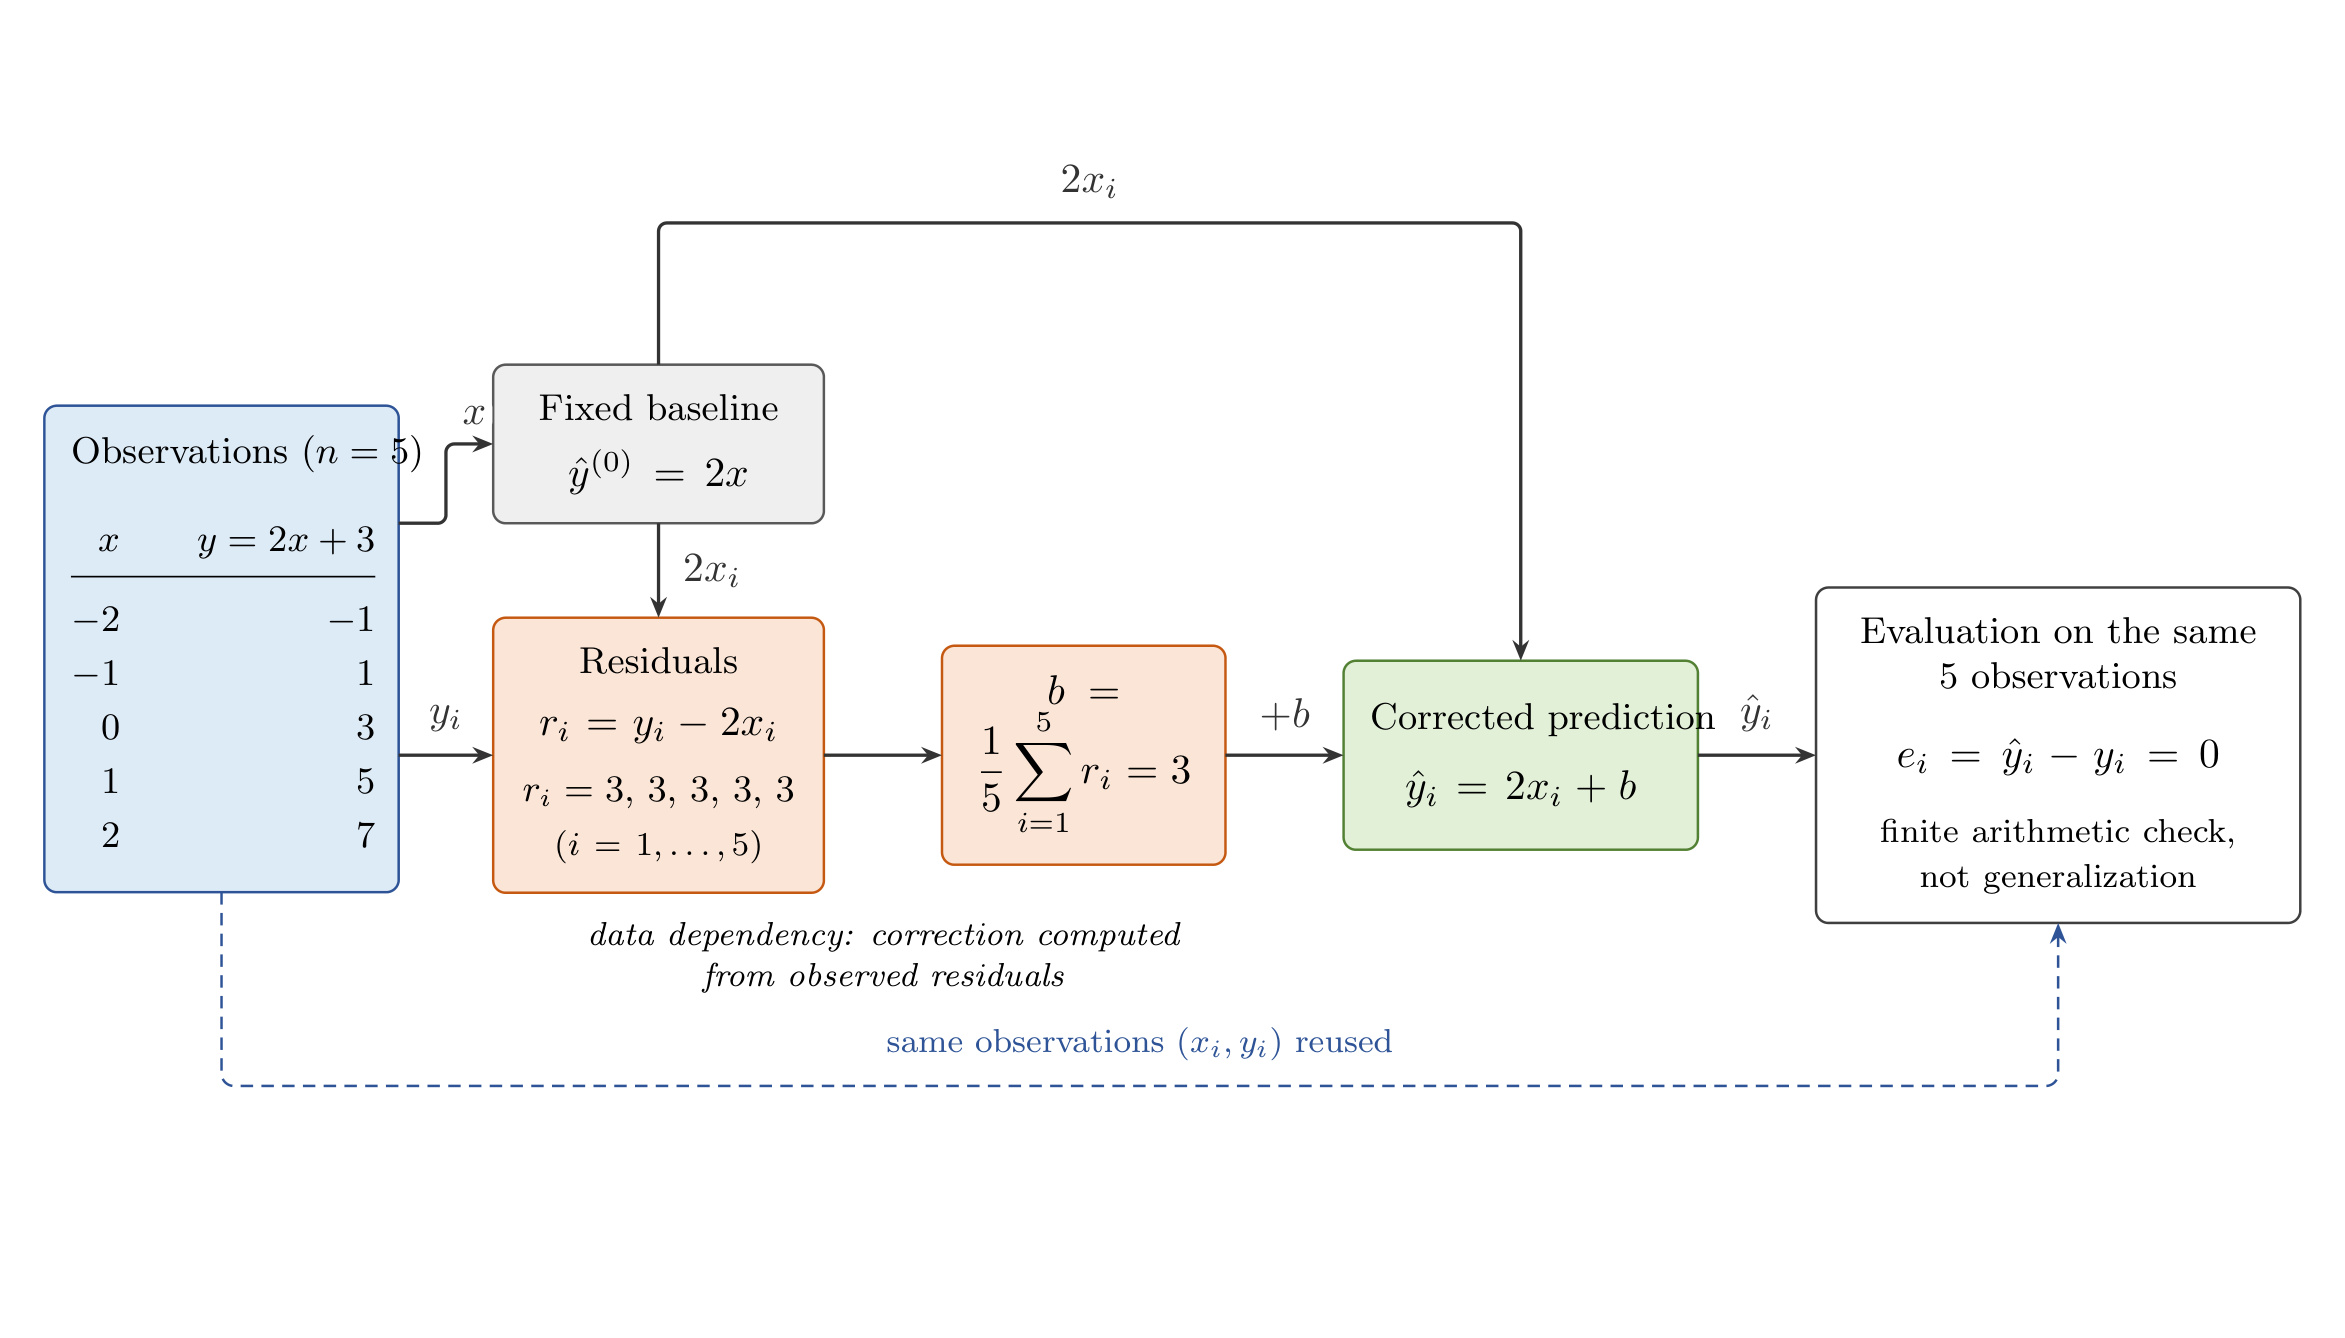
\includegraphics[width=\linewidth]{figures/fig_residual_workflow.jpg}
    \caption{Fitting and scoring dependencies. Solid arrows trace the correction; the dashed path identifies the observations reused for scoring. The baseline residual is target minus prediction; the diagram's corrected error is prediction minus target.}
    \label{fig_residual_workflow}
\end{figure}

\subsection{Error Definitions and Reproducible Calculation}

The baseline residual $r_i$ is the amount missing from the baseline prediction. Following Figure~\ref{fig_residual_workflow}, corrected error measures the amount by which prediction exceeds target:
\[
e_i(b)=\hat y_i(b)-y_i=b-r_i.
\]
For the supplied residuals,
\begin{align}
\operatorname{MAE}(b)
&=\frac{1}{5}\sum_{i=1}^{5}|e_i(b)|=|b-3|,
\label{eq:mae}\\
\operatorname{MSE}(b)
&=\frac{1}{5}\sum_{i=1}^{5}e_i(b)^2=(b-3)^2.
\label{eq:mse}
\end{align}
Absolute values and squares remove the sign difference.

For five arbitrary ordered residuals, let
$C=(r_{(5)}-r_{(1)})+(r_{(4)}-r_{(2)})$.
Pairing extremes gives the complete bound
\[
\sum_{i=1}^{5}|b-r_{(i)}|
\geq C+|b-r_{(3)}|
\geq C.
\]
Each paired bound is attained when $b$ lies between its endpoints. At $b=r_{(3)}$, both pairs attain equality and the middle term vanishes. Every other $b$ makes the middle term positive, establishing the unique minimizer.

The same pairing argument gives the middle residual for any odd sample size. For $n=2k$,
\[
\sum_{i=1}^{2k}|b-r_{(i)}|
\geq
\sum_{i=1}^{k}\bigl(r_{(2k+1-i)}-r_{(i)}\bigr).
\]
Equality holds precisely in the intersection of all paired intervals,
$[r_{(k)},r_{(k+1)}]$, which is the full minimizing set.

For five arbitrary residuals and any median $m$, Equation~\ref{eq:decomposition} gives
$\operatorname{MSE}(m)-\operatorname{MSE}(\bar r)=(m-\bar r)^2$,
whereas $\operatorname{MAE}(m)\leq\operatorname{MAE}(\bar r)$.
These statements distinguish the objectives algebraically. The supplied vector makes both corrections equal $3$.

\section{Experiments}
\subsection{Observations and Evaluation Protocol}

The supplied observation rows are
\[
\begin{array}{c|rrrrr}
x & -2 & -1 & 0 & 1 & 2\\
y & -1 & 1 & 3 & 5 & 7\\
2x & -4 & -2 & 0 & 2 & 4\\
2x+3 & -1 & 1 & 3 & 5 & 7
\end{array}
\]
One deterministic R calculation \cite{Ihaka1996RLanguage} evaluates $b=0$, $1.5$, and $3$. The same targets determine the fitted correction and enter scoring. Apparent error therefore establishes agreement on these specified observations.

To assess predictions on separate observations $(x_j^*,y_j^*)$, the fitted correction would remain fixed at $3$: predictions would be $2x_j^*+3$, with evaluation targets entering only the error summaries. This separates estimating the correction from assessing its predictions.

\subsection{Recorded Errors and Their Interpretation}

Subtracting baseline predictions from targets gives $(3,3,3,3,3)$, with sum $15$ and mean $3$. Corrected errors have constant entries $-3$, $-1.5$, and $0$ at the recorded corrections. Their absolute values and squares give Table~\ref{tab_recorded_errors}.

\begin{table}[!htbp]
    \centering
    \caption{Computed apparent errors on the five supplied observations.}
    \label{tab_recorded_errors}
    \begin{tabular}{@{}rrr@{}}
        \toprule
        Added $b$ & Mean absolute error & Mean squared error\\
        \midrule
        0   & 3   & 9\\
        1.5 & 1.5 & 2.25\\
        3   & 0   & 0\\
        \bottomrule
    \end{tabular}
\end{table}

\begin{figure}[!htbp]
    \centering
    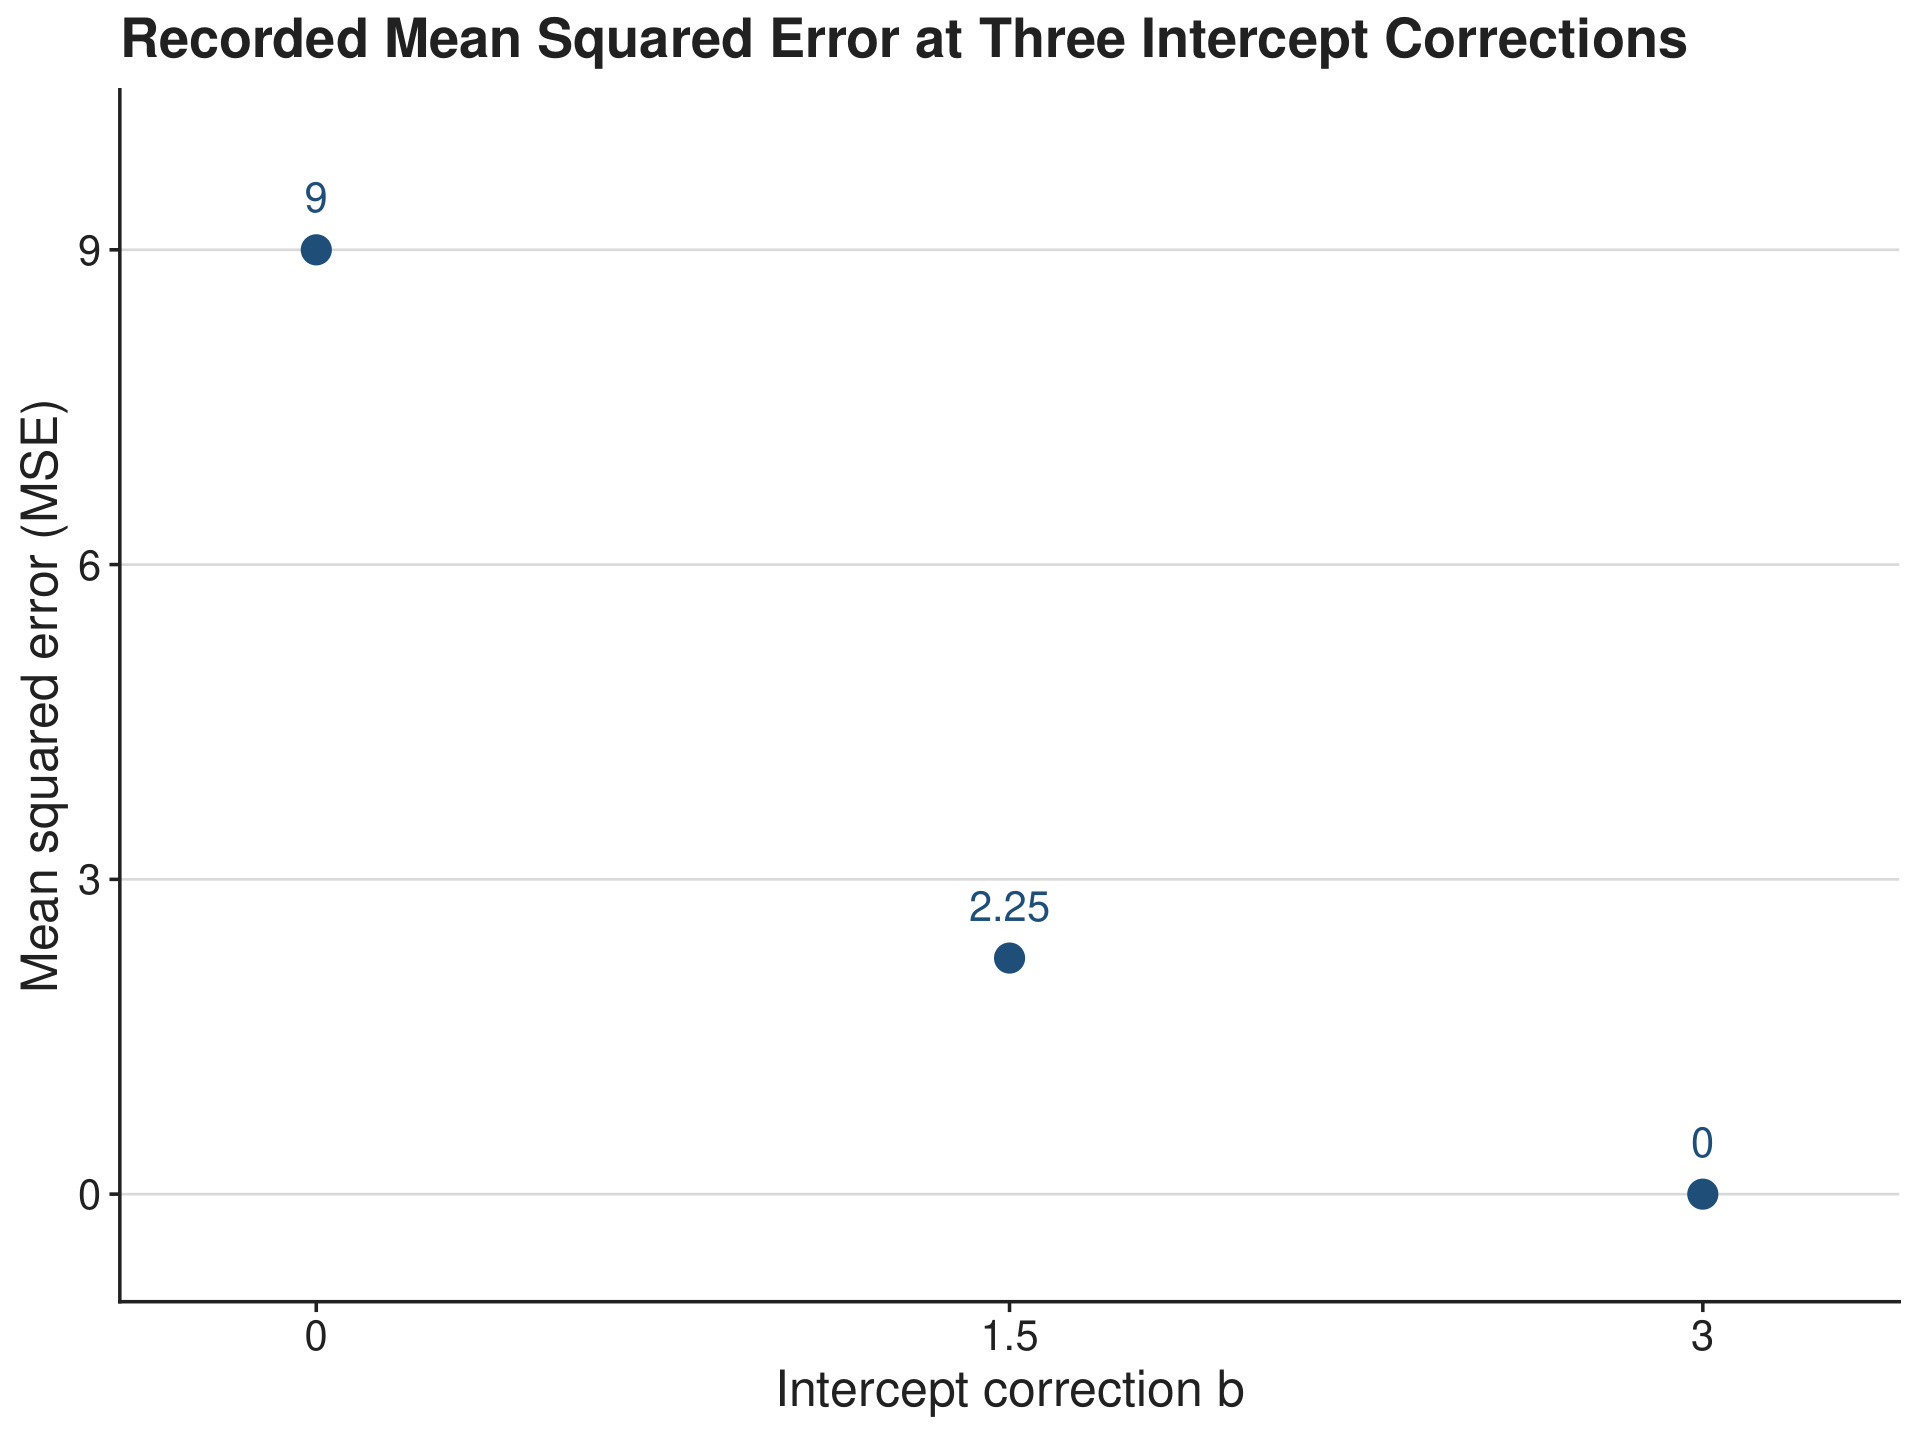
\includegraphics[width=0.8\linewidth]{figures/fig_intercept_error.jpg}
    \caption{The three recorded MSE values: $(0,9)$, $(1.5,2.25)$, and $(3,0)$. Each labeled point corresponds to one table row.}
    \label{fig_intercept_error}
\end{figure}

The bundled R/ggplot2 source \cite{Wickham2009LayeredGrammar} explicitly stores these three coordinate pairs; the manuscript table transcribes the same experimental record. Their agreement checks transcription. The observation-based arithmetic above independently derives the values.

Both figure sources accompany the submission, together with rendering metadata, the plot export wrapper, and the checksum manifest identified below. Checksums identify artifact versions; equations and observation rows establish the numerical checks.

\section{Conclusion}

This finite exercise links a fitted intercept, its loss function, and its scoring dependencies. Separate proofs identify the mean and median corrections; constant residuals explain their shared value and exact agreement here. The audit sequence connects those mathematical statements to inspectable observations, figures, and reported errors.

\bibliographystyle{plain}
\bibliography{references}

% PAPER_ORCHESTRA_PROVENANCE_BEGIN
\clearpage
\section*{Figure source provenance}
The files below are the exact sources that produced the embedded figure previews. Paths are relative to this manuscript's source directory. The accompanying \texttt{figure\char95{}provenance.json} records all artifact checksums.\par
\medskip\noindent\textbf{Figure~\ref{fig_intercept_error} (\texttt{fig\char95{}intercept\char95{}error.jpg}).}\par
\noindent R/ggplot2 source: \texttt{figure\char95{}code/\allowbreak{}fig\char95{}intercept\char95{}error/\allowbreak{}source.R}.\par
\noindent Source SHA256: \texttt{68963e7e\allowbreak{}0f21eaa5\allowbreak{}7dfe9d41\allowbreak{}50f6248f\allowbreak{}d142e763\allowbreak{}e30835f3\allowbreak{}e6e8af10\allowbreak{}adc25ae2}.\par
\noindent Rendering metadata: \texttt{figure\char95{}code/\allowbreak{}fig\char95{}intercept\char95{}error/\allowbreak{}render.json}.\par
\noindent Exact export wrapper: \texttt{figure\char95{}code/\allowbreak{}fig\char95{}intercept\char95{}error/\allowbreak{}worker.R}.\par
\noindent Wrapper SHA256: \texttt{6cb2b073\allowbreak{}27277f63\allowbreak{}fafbb553\allowbreak{}cd4f1f12\allowbreak{}c0f85bec\allowbreak{}37a49f3f\allowbreak{}a765da16\allowbreak{}a26b58ba}.\par
\noindent Rendering metadata: \texttt{figure\char95{}code/\allowbreak{}fig\char95{}intercept\char95{}error/\allowbreak{}sessionInfo.txt}.\par
\medskip\noindent\textbf{Figure~\ref{fig_residual_workflow} (\texttt{fig\char95{}residual\char95{}workflow.jpg}).}\par
\noindent LaTeX/TikZ source: \texttt{figure\char95{}code/\allowbreak{}fig\char95{}residual\char95{}workflow/\allowbreak{}source.tex}.\par
\noindent Source SHA256: \texttt{66606680\allowbreak{}7053c57a\allowbreak{}dee8b194\allowbreak{}7e99adeb\allowbreak{}6a9369c3\allowbreak{}c53399fd\allowbreak{}76a38033\allowbreak{}1907dee2}.\par
\noindent Rendering metadata: \texttt{figure\char95{}code/\allowbreak{}fig\char95{}residual\char95{}workflow/\allowbreak{}render.json}.\par
% PAPER_ORCHESTRA_PROVENANCE_END
\end{document}